\chapter{Atividades Desenvolvidas}\label{sec:ativ_desenvolvidas}
Nesta seção, é apresentada, em detalhes, cada uma das principais atividades realizadas para a condução deste projeto.

\section{Estudos sobre usabilidade e acessibilidade}\label{sec:estudos_usab_acess} 

% O que é acessibilidade em termos gerais 
% Em termos digitais (Towards a unified definition of web accessibility. the 12th Web for all Conference, ACM, 2015, p. 35.)

% Falar que alguns softwares e aplicativos impossibilitam o uso de um certo público

% Falar da wcag como uma forma de combater isso
 Segundo a Lei 10.098, de 19 de dezembro de 2000 da Legislação Brasileira, a acessibilidade é a possibilidade e condição de alcance para utilização, com segurança e autonomia, dos
espaços, mobiliários e equipamentos urbanos, das
edificações, dos transportes e dos sistemas e meios de comunicação por pessoa portadora de deficiência ou com mobilidade reduzida. \cite{torres2002acessibilidade} diz que acessibilidade é um processo dinâmico, associado não só ao desenvolvimento tecnológico, mas principalmente ao desenvolvimento da sociedade. Em geral, está associada a pessoas com deficiências físicas ou psicológicas, idosos ou grupos excluídos; este último mais bem relacionado com o termo \textit{inclusão}. Embora a acessibilidade não se restrinja ao meio digital, é essencial que esteja presente no mesmo. Corroborando com essa ideia, \cite{leew3c} afirma a importância da Web ser utilizável por qualquer um, independente de capacidades individuais ou deficiências. No atual panorama isso também se aplica ao uso de aplicativos em dispositivos móveis. 

Atrelada à acessibilidade deve estar a usabilidade, que segundo \cite{nielsenPrioritizingWebUsability}
é o atributo relacionado a quão fácil é usar algo. Mais especificamente, refere-se a quão rápido pessoas podem aprender a usar algo, quão eficientes são enquanto o utilizam, quão memorável é, quão propenso a erros e o quanto as pessoas gostam de utilizar. Deve-se tornar a utilização fluida, a frase ''não me faça pensar`` deve ser aplicada ao usuário.
Ademais, é essencial analisar fatores como capacidade de aprendizagem, a fim de que não seja necessário um aprendizado extra por parte do usuário para utilizar o sistema em questão. Isso seria um problema pois escaparia do objetivo principal do projeto.

% Falar que o problema se aplica a idosos no final da seção
No contexto em que se insere esse projeto isso se torna ainda mais essencial, uma vez que o público idoso sofre bastante com a usabilidade em \textit{smartphones} \citep{dificuldadesIdosos}.  

\section{Estudo sobre Aprendizagem móvel}\label{sec:estudos_ap_movel} 
Nesta seção serão abordados o conceito de aprendizagem móvel bem como uma pesquisa das principais funcionalidades presentes em aplicativos relacionados ao ensino, de palavras cruzadas e relacionados ao idoso.

\subsection{Panorama}
Existem várias definições de \textit{m-learning}. Ao longo dos anos, pesquisadores se dispuseram a estudar o assunto e tentaram achar uma definição. De acordo com \cite{Quinn2000}, \textit{m-learning} é um modelo de aprendizagem eletrônica (\textit{e-learning}) que utiliza equipamentos computadorizados: \textit{Palmtops}, dispositivos que rodam Windows Embedded Compact e até um telefone celular.
Em 2011, \cite{hwang2011research} disseram que uma definição amplamente aceita de \textit{m-learning} é simplesmente ``usar tecnologias móveis para facilitar o aprendizado''. Dentre outras definições, a adotada para esse projeto foi a seguinte: qualquer fornecimento educacional onde a tecnologia dominante é portátil ou dispositivos \textit{palmtop} \citep{traxler2005defining}.

Todavia, independente da definição tomada, torna-se necessário analisar vantagens e desvantagens de utilizar dispositivos móveis. De acordo com \cite{RICHAMEHTA2016} destacam-se como vantagens: (i) PDAs ou tablets com anotações e e-books são mais leves e menos volumosos que mochilas cheias de papéis, livros e até laptops; (ii) É mais fácil acomodar dispositivos móveis em uma sala se comparado à computadores de mesa; (iii) Dispositivos móveis podem ser usados em qualquer lugar e em qualquer momento, como em trens, em casa, em hotéis. Isto tem um valor inestimável para a educação \citep{CarmaMaia2008}.

De acordo com \cite{RICHAMEHTA2016}, destacam-se as seguintes desvantagens: (i) Celulares pequenos e telas de PDAs limitam-se a quantidade e tipo de informação que pode ser exibida; (ii) Baterias precisam ser recarregadas regularmente, e dados podem ser perdidos caso não se faça o carregamento correto; (iii) É difícil usar gráficos que possuem movimento, especialmente em celulares pequenos.

Devido ao processo de envelhecimento, limitações e desafios podem ser potencializadas no caso de usuários idosos, visto que podem ocorrer mudanças para o idoso durante esse processo. Além disso, é necessário que as aplicações educacionais móveis levem em consideração propostas pedagógicas adequadas e específicas para esse público. Desse modo, é indispensável que o desenvolvimento dessas aplicações seja realizado de maneira clara e objetiva, possibilitando melhor aprendizagem por parte do idoso.

\subsection{Pesquisa sobre as principais funcionalidades de aplicativos de aprendizagem móvel}
Diversos são os aplicativos que possuem o objetivo de apoiar o processo de ensino e aprendizagem do usuário; seja por meio de jogos, vídeos ou outros materiais. Dessa maneira, alguns aplicativos (para diferentes públicos) foram analisados, a fim de verificar suas funcionalidades e propostas de aprendizagem e acessibilidade, de maneira que essas pudessem ser adaptadas ou utilizadas para aplicações com foco no idoso.

\begin{description}
% Ensina o que? Qual o publico alvo? Pessoas de quantos anos?

\item[Engaging congress]\footnote{\url{https://play.google.com/store/apps/details?id=com.iu.engagingcongress&hl=en}, \url{https://apps.apple.com/us/app/engaging-congress/id1309161238?ls=1}} \hfill \\
\textit{Enganging congress} (\autoref{fig:EngCong}) é um jogo interativo que visa explorar os princípios básicos de um governo representativo. Escolhe-se um tema e é exibido um vídeo. Jogos são incluídos no processo baseados no tema. É importante destacar a atenção dos criadores em fazer o usuário compreender a tarefa; a todo momento é possível clicar no botão de dúvida. As principais funcionalidades são: (i) vídeos educativos sobre o tema; (ii) perguntas relacionadas ao conteúdo passado; (iii) nota final após a conclusão dos exercícios; (iv) botões de dúvidas sempre presentes.

\begin{figure}[ht!]
\centering
    \caption{Telas do aplicativo \textit{Engaging Congress}}
    \label{fig:EngCong}
    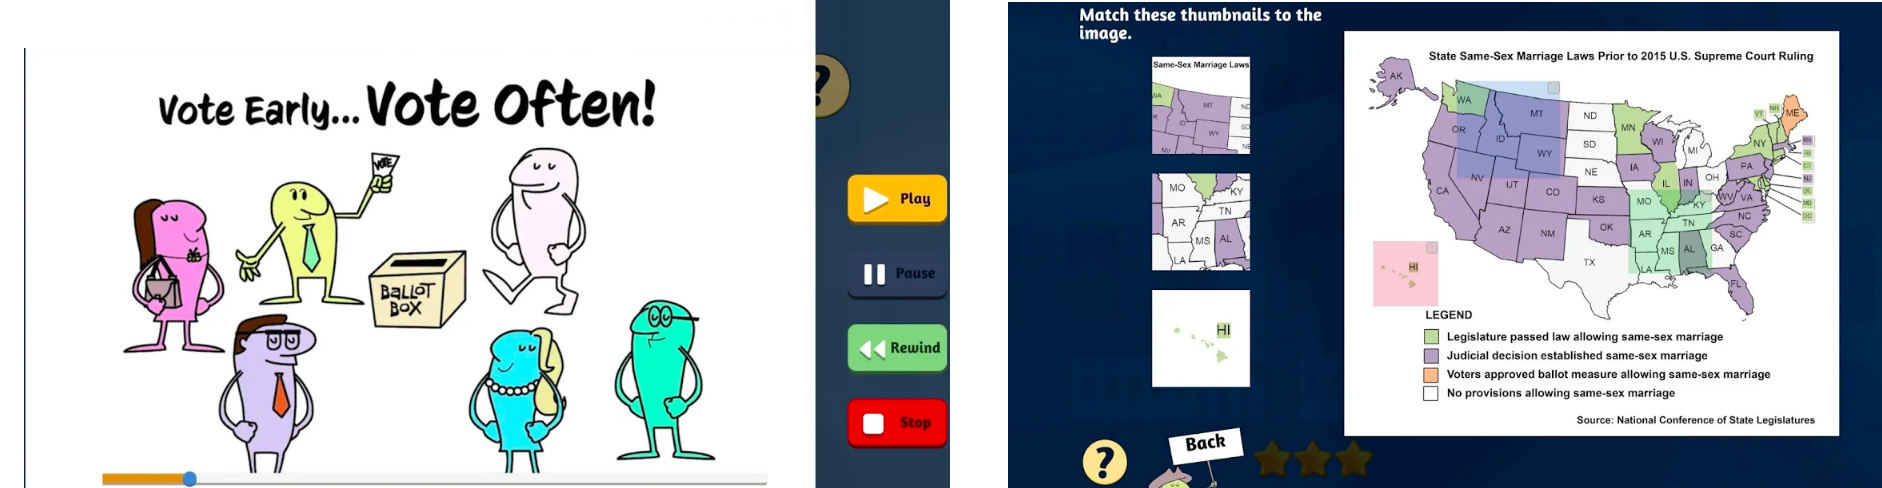
\includegraphics[width=0.9\textwidth]{Figuras/engagingcongress.png}
    
    Fonte: Elaborada pelo autor
\end{figure}

\item[Play PBS KIDS Games]\footnote{\url{https://apps.apple.com/us/app/pbs-kids-games/id1050773989}, \url{https://play.google.com/store/apps/details?id=org.pbskids.gamesapp&hl=pt_BR}} \hfill \\
O aplicativo (\autoref{fig:pbs}) visa a promoção da educação para crianças na fase de alfabetização (2 a 8 anos), pois contém mais de 100 mini-jogos voltados para tal. As crianças são encorajadas a resolver desafios e aprimorar suas habilidades em ciências, matemática, letras e criatividade. O objetivo é impactar positivamente as vidas de crianças por meio de mídia baseada em um currículo onde quer que elas estejam. O app ganhou duas premiações no ano de 2017, a saber Melhor aplicativo de jogos para Pré-Escola (\textit{Kidscreen Award Winner}) e o \textit{Parents' Choice Recommended Mobile App}. Os principais recursos são: (i) funcionamento offline; (ii) possibilidade de gerenciar a quantidade de memória que será consumida; (iii) obter detalhes sobre desenhos da TV PBS Kids como idade recomendada e objetivos de aprendizado para as crianças.

\begin{figure}[H]
\centering
    \caption{Telas do aplicativo \textit{Play PBS KIDS Games}}
    \label{fig:pbs}
    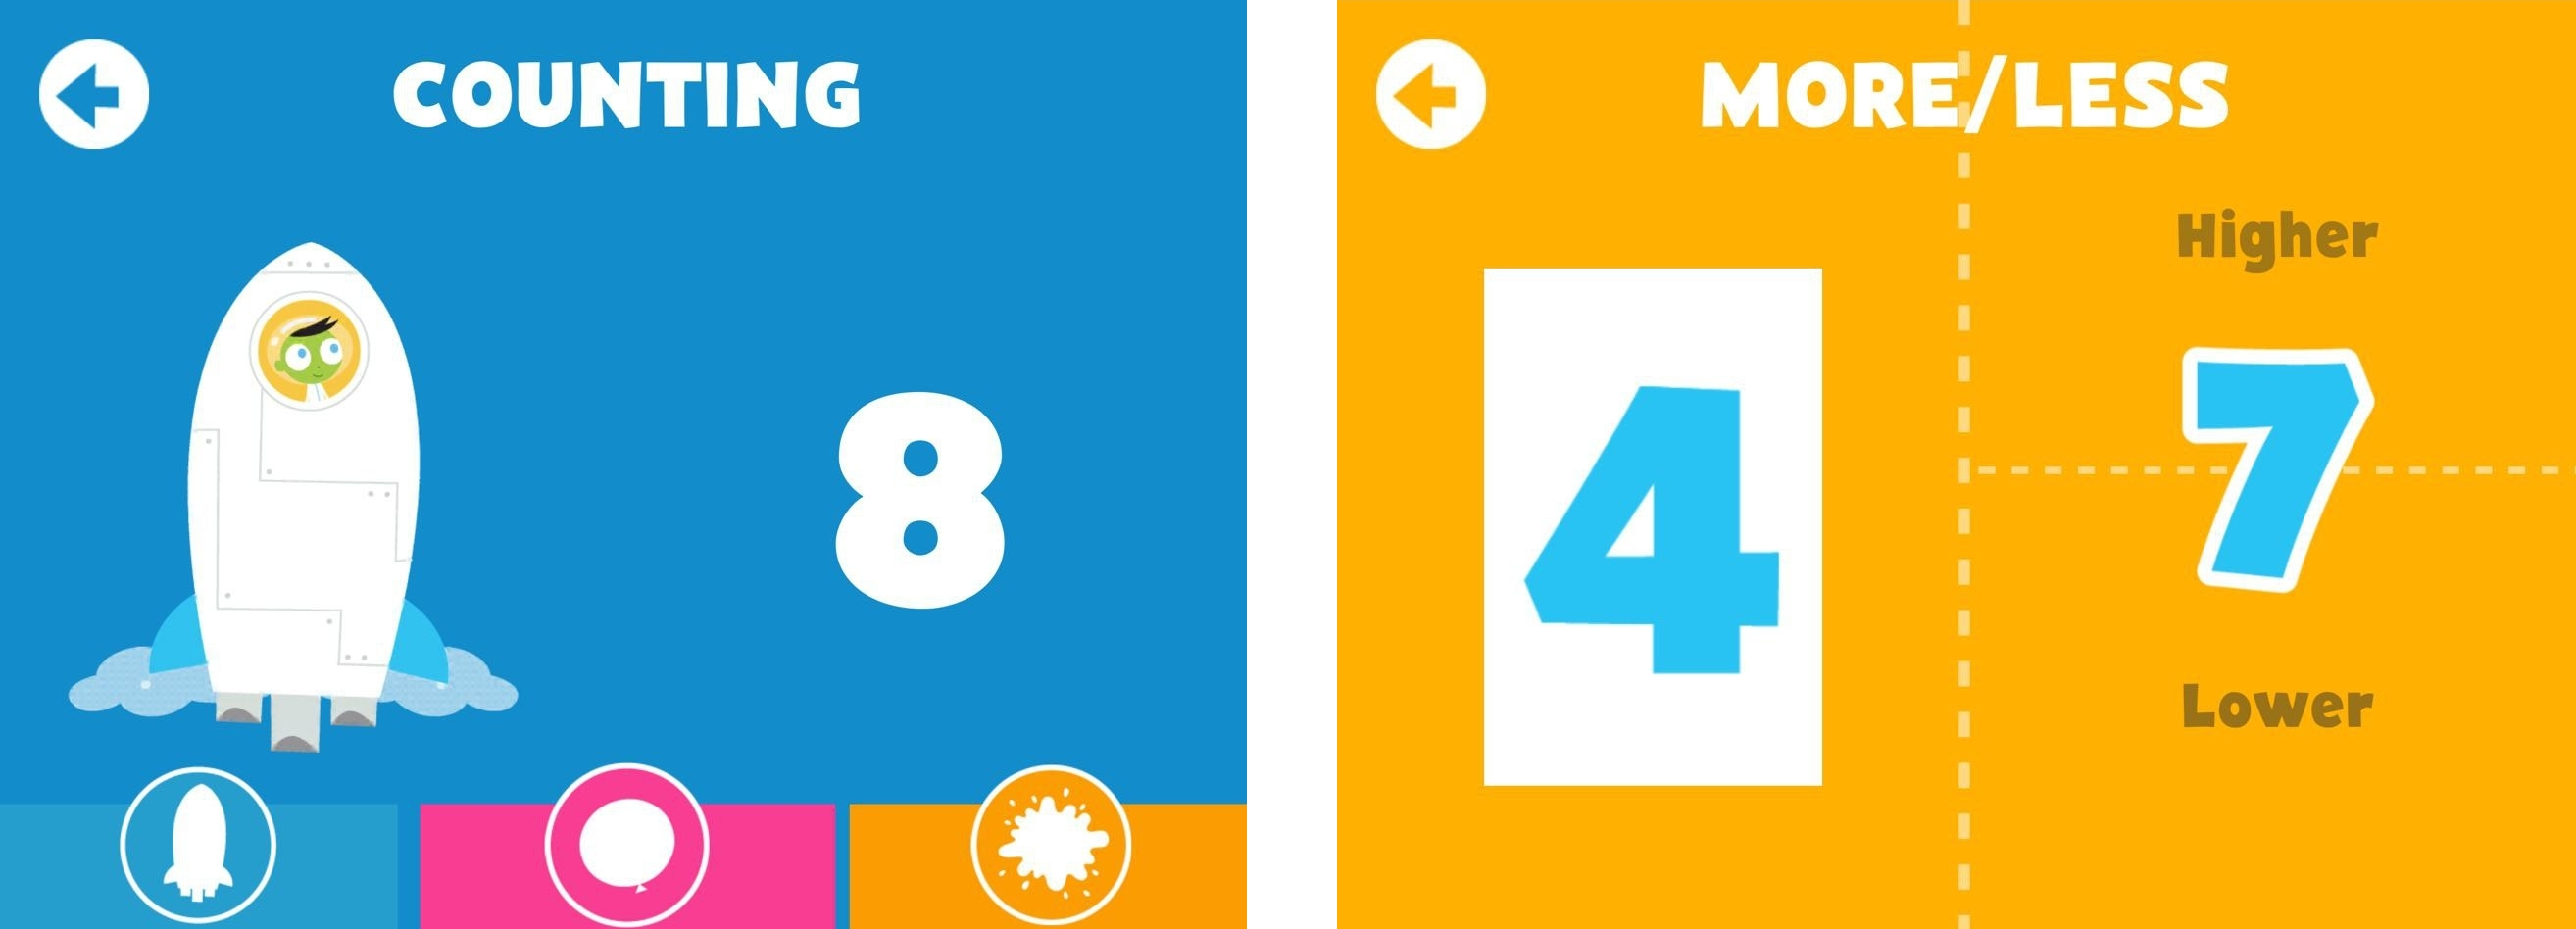
\includegraphics[width=0.9\textwidth]{Figuras/pbsKids.jpg}
    
    Fonte: Elaborada pelo autor
\end{figure}

\item[Human Anatomy Atlas]\footnote{\url{https://apps.apple.com/br/app/human-anatomy-atlas-2020/id1117998129}, \url{https://play.google.com/store/apps/details?id=com.argosy.vbandroid&hl=pt_BR}} \hfill \\
O \textit{Human Anatomy Atlas} (\autoref{fig:humAtlas}) é um aplicativo criado por um time de especialistas em visualização biomédica. É direcionado ao ensino da anatomia do corpo humano com o foco em estudantes e professores, apesar de também ser utilizado em hospitais. Seus modelos em 3D promovem uma fidelidade às estruturas humanas reais, sendo possível rotacionar e dissecar órgãos e partes do corpo. Possui recursos como : (i) interatividade com estruturas 3D; (ii) mais de 1000 questões para testes em assuntos; (iii) visualização de anatomias complexas em realidade aumentada; (iv) disponibilidade em 7 idiomas.

\begin{figure}[ht!]
\centering
    \caption{Telas do aplicativo \textit{Human Anatomy Atlas}}
    \label{fig:humAtlas}
    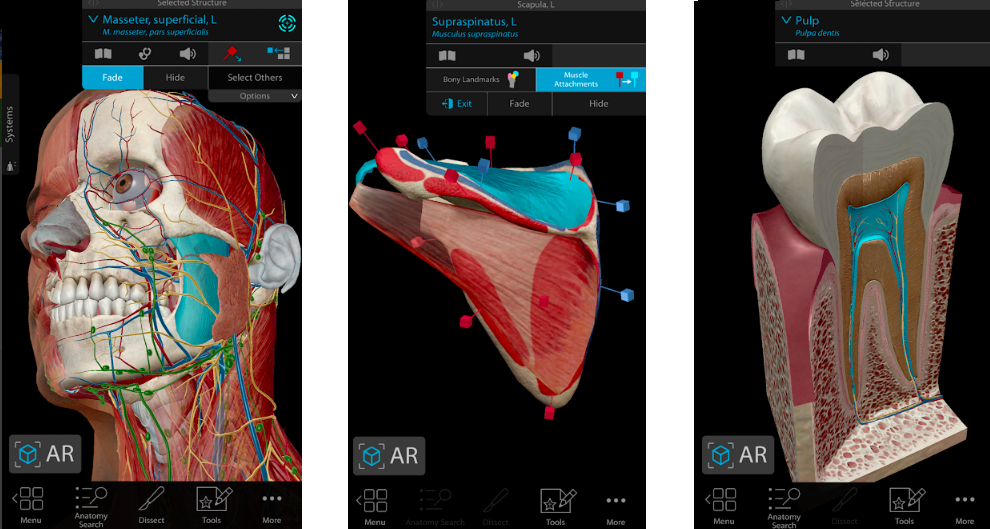
\includegraphics[width=0.9\textwidth]{Figuras/humanAtlas.png}
    
    Fonte: \cite{HumanAnatomyAtlas}
\end{figure}

\item[Bini Super ABC]\footnote{\url{https://apps.apple.com/br/app/bini-abc-alfabeto-crianças-app/id1397966958}, \url{https://play.google.com/store/apps/details?id=com.binibambini.abc&hl=pt_BR}} \hfill \\
Bini Super ABC (\autoref{fig:biniABC}) é um aplicativo voltado para crianças na faixa de 3 a 5 anos na fase de instrução educacional. O aplicativo promove o aprendizado das letras do alfabeto com diversos jogos infantis. O objetivo é tornar o ensino interessante e empolgante com desenhos coloridos, personagens e efeitos sonoros. A aplicação possui as funcionalidades: (i) aprendizado das letras por sons; (ii) reforço do material aprendido; (iii) controle de responsáveis para os jogos.

\begin{figure}[H]
\centering
    \caption{Telas do aplicativo \textit{Bini Super ABC}}
    \label{fig:biniABC}
    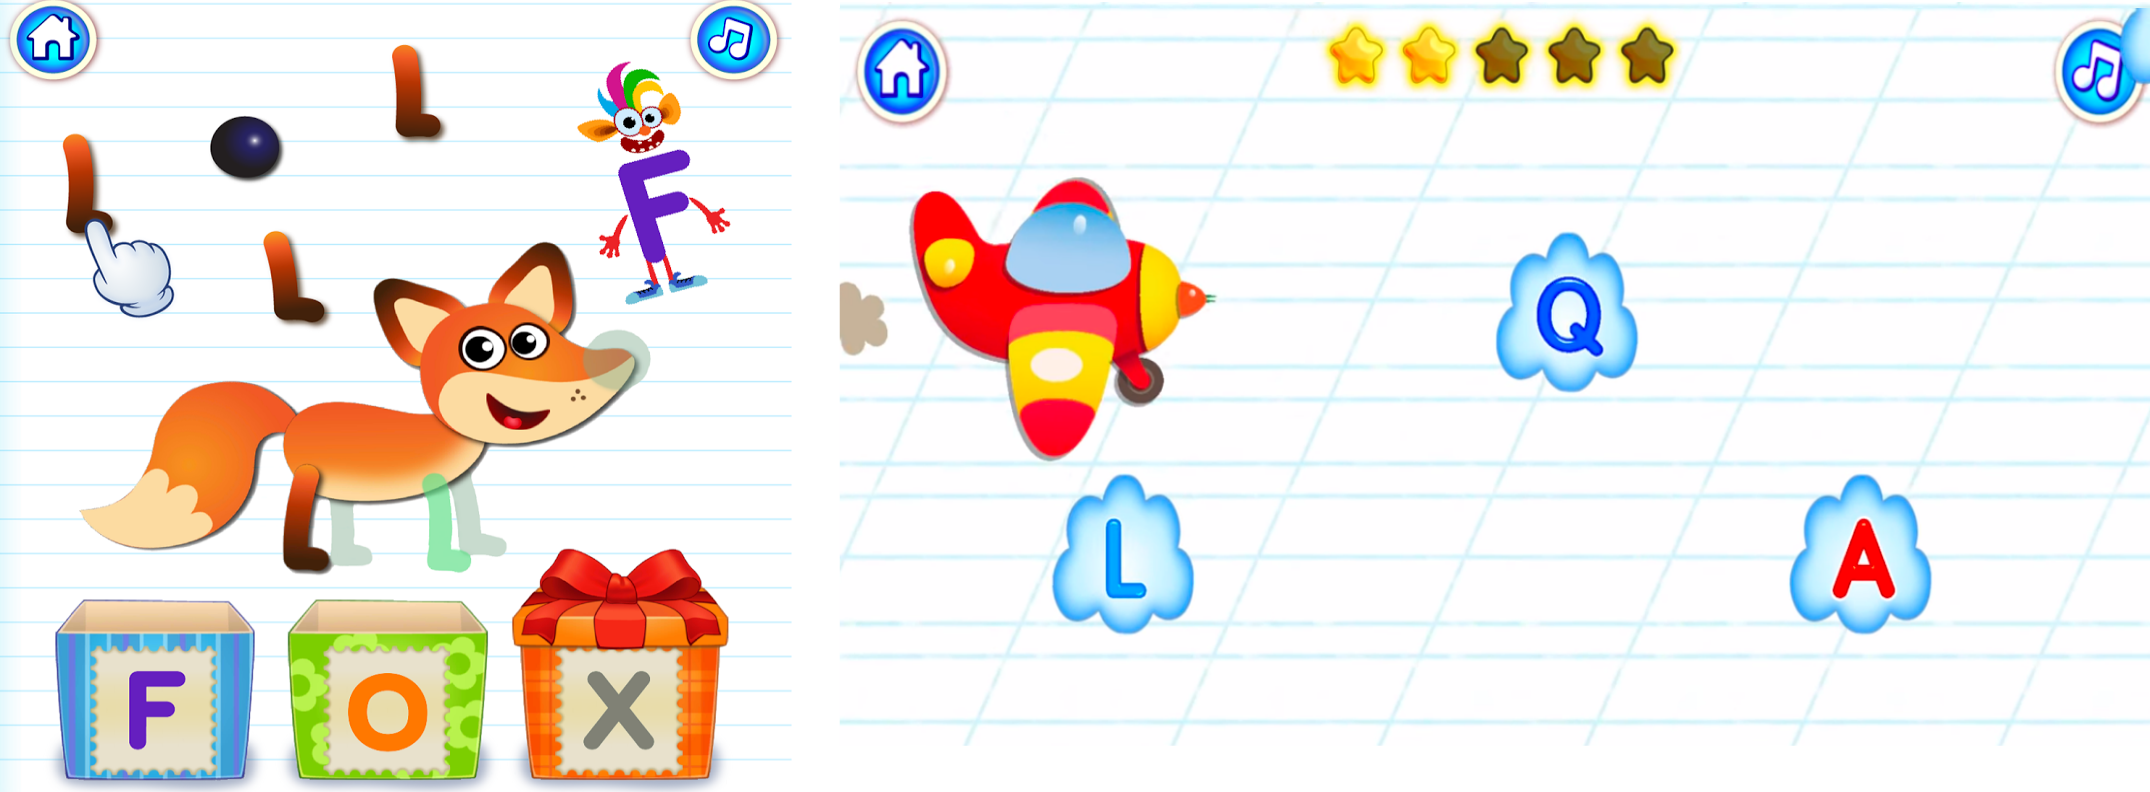
\includegraphics[width=0.9\textwidth]{Figuras/biniabc.png}
    
    Fonte: Elaborada pelo autor
\end{figure}

\item[Crossword Puzzle Free]\footnote{\url{https://play.google.com/store/apps/details?id=mobi.redstonegames.crossword.en&hl=pt_BR}} \hfill \\
Crossword Puzzle Free (\autoref{fig:crossFree}) é um aplicativo de palavras cruzadas. É simples e fácil de usar não exigindo conhecimentos específicos do usuário. Com os 4 níveis de dificuldade é possível buscar o desafio na medida certa além de motivar o usuário a continuar utilizando o aplicativo por não ser nem muito fácil nem muito difícil. As principais funcionalidade são: (i) Teclado do próprio aplicativo; (ii) Dicas aparecem acima do teclado; (iii) Botão de dica para a palavra.


\begin{figure}[H]
\centering
    \caption{Telas do aplicativo \textit{Crossword Puzzle Free}}
    \label{fig:crossFree}
    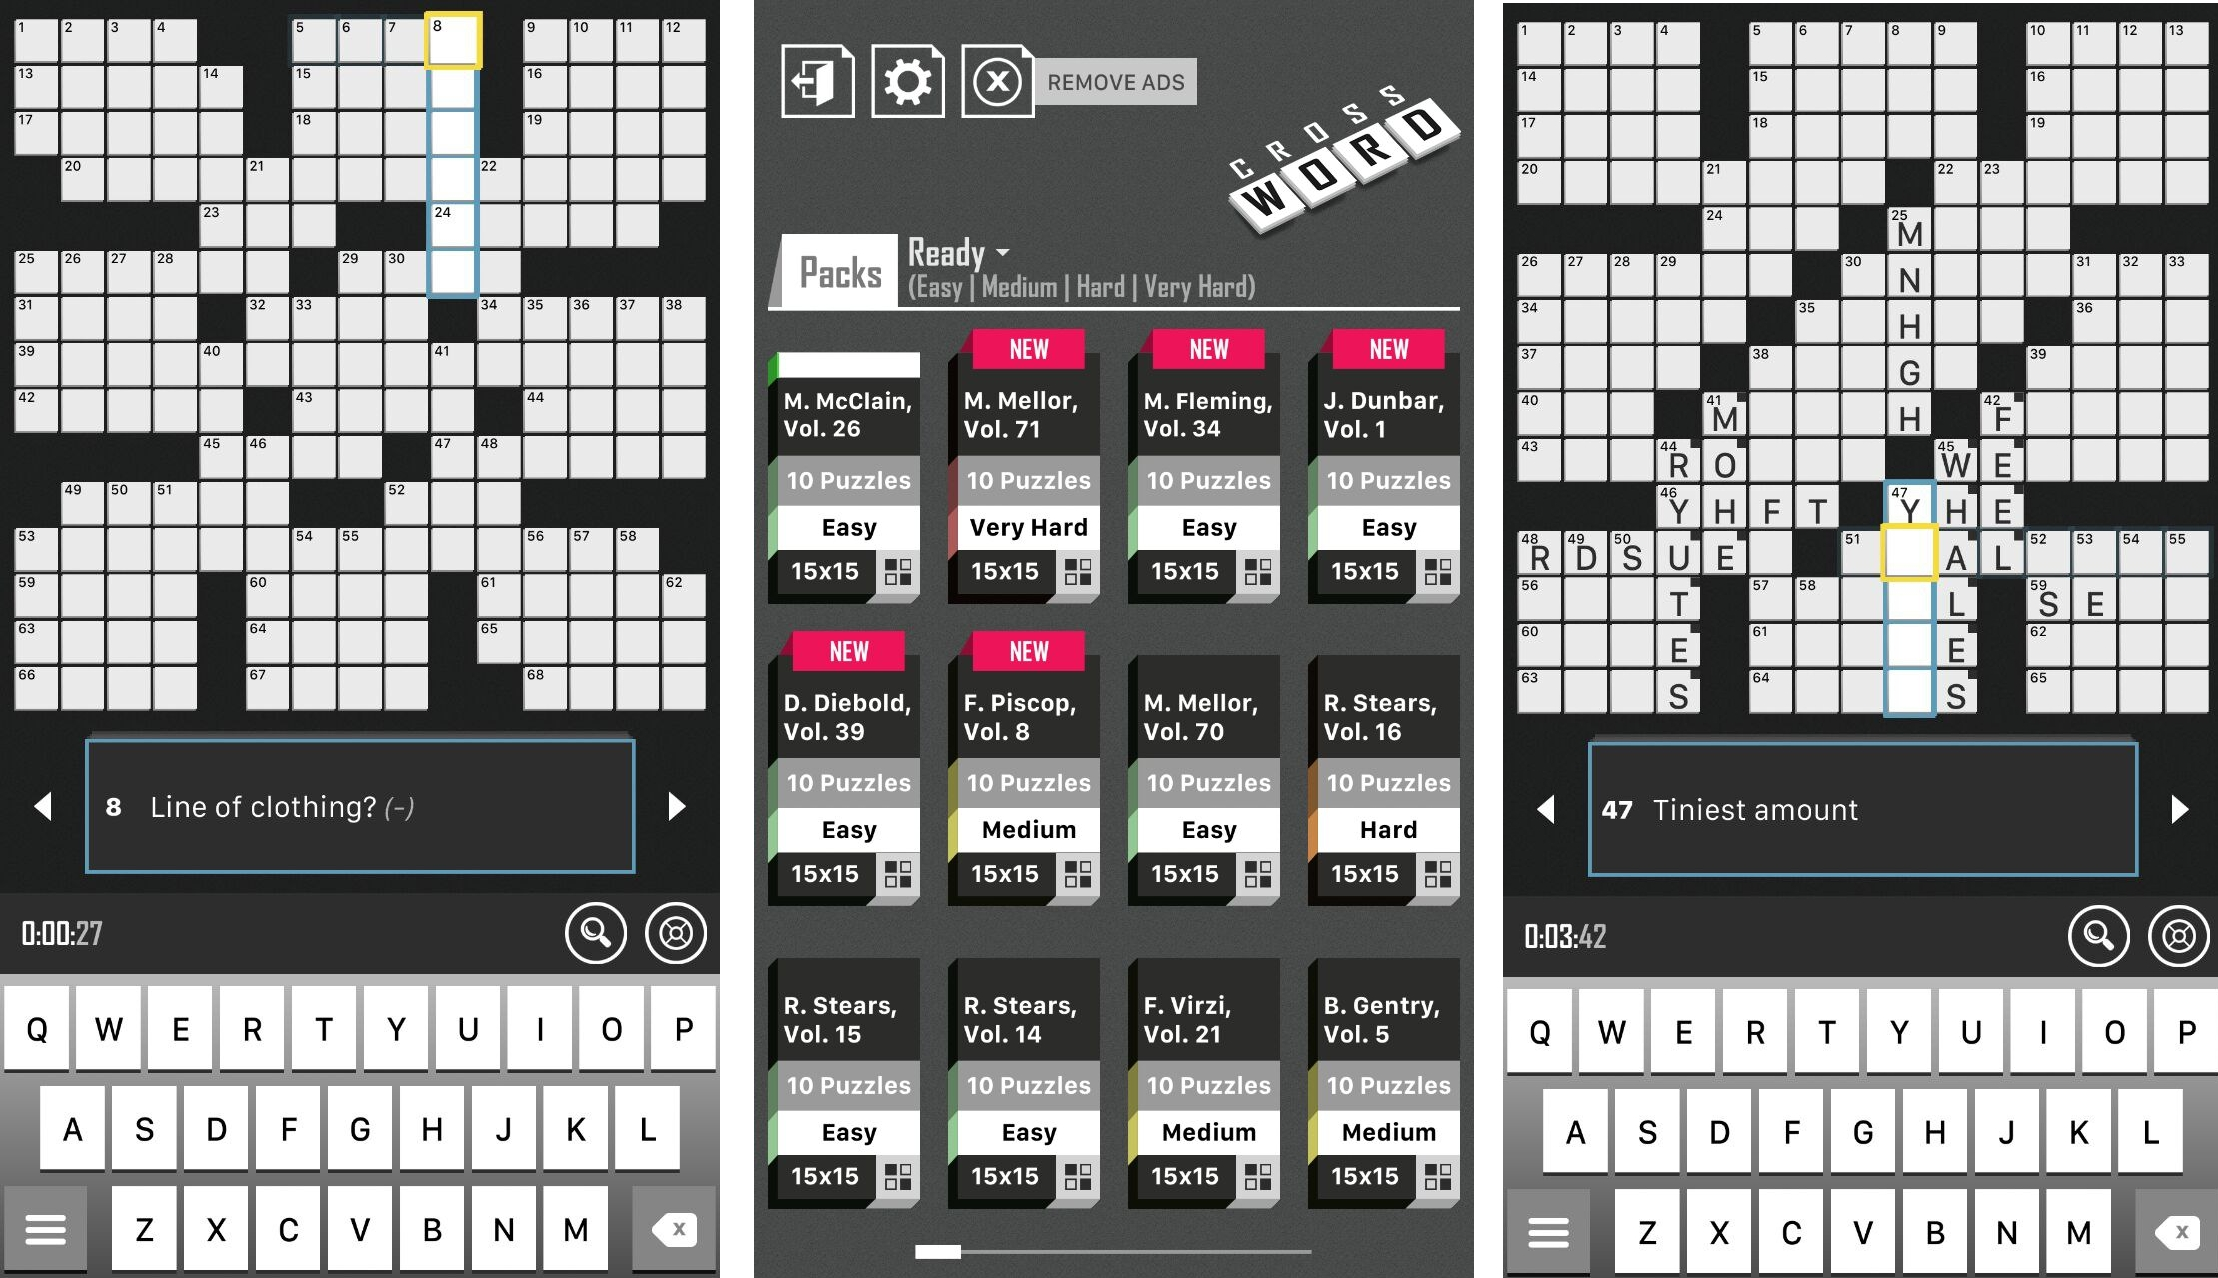
\includegraphics[width=0.9\textwidth]{Figuras/crosswordPuzzleFree.jpg}
    
    Fonte: Elaborada pelo autor
\end{figure}

\item[Crossword Quiz]\footnote{\url{https://play.google.com/store/apps/details?id=com.randomlogicgames.crossword&hl=pt_BR}} \hfill \\
Crossword Quiz (\autoref{fig:crossQuiz}) é um aplicativo de palavras cruzadas com uma abordagem mais fácil por não disponibilizar todas as letras do teclado, tornando a resposta mais fácil para o usuário. Além disso, o aplicativo não conta apenas com dicas escritas, mas inclui imagens. As funcionalidade que se destacam são: (i) Não mostrar todo o teclado, apenas algumas letras; (ii) Mostra imagens como dicas além de textos; (iii) Tutorial inicial intuitivo e completo.

\begin{figure}[H]
\centering
    \caption{Telas do aplicativo \textit{Crossword Quiz}}
    \label{fig:crossQuiz}
    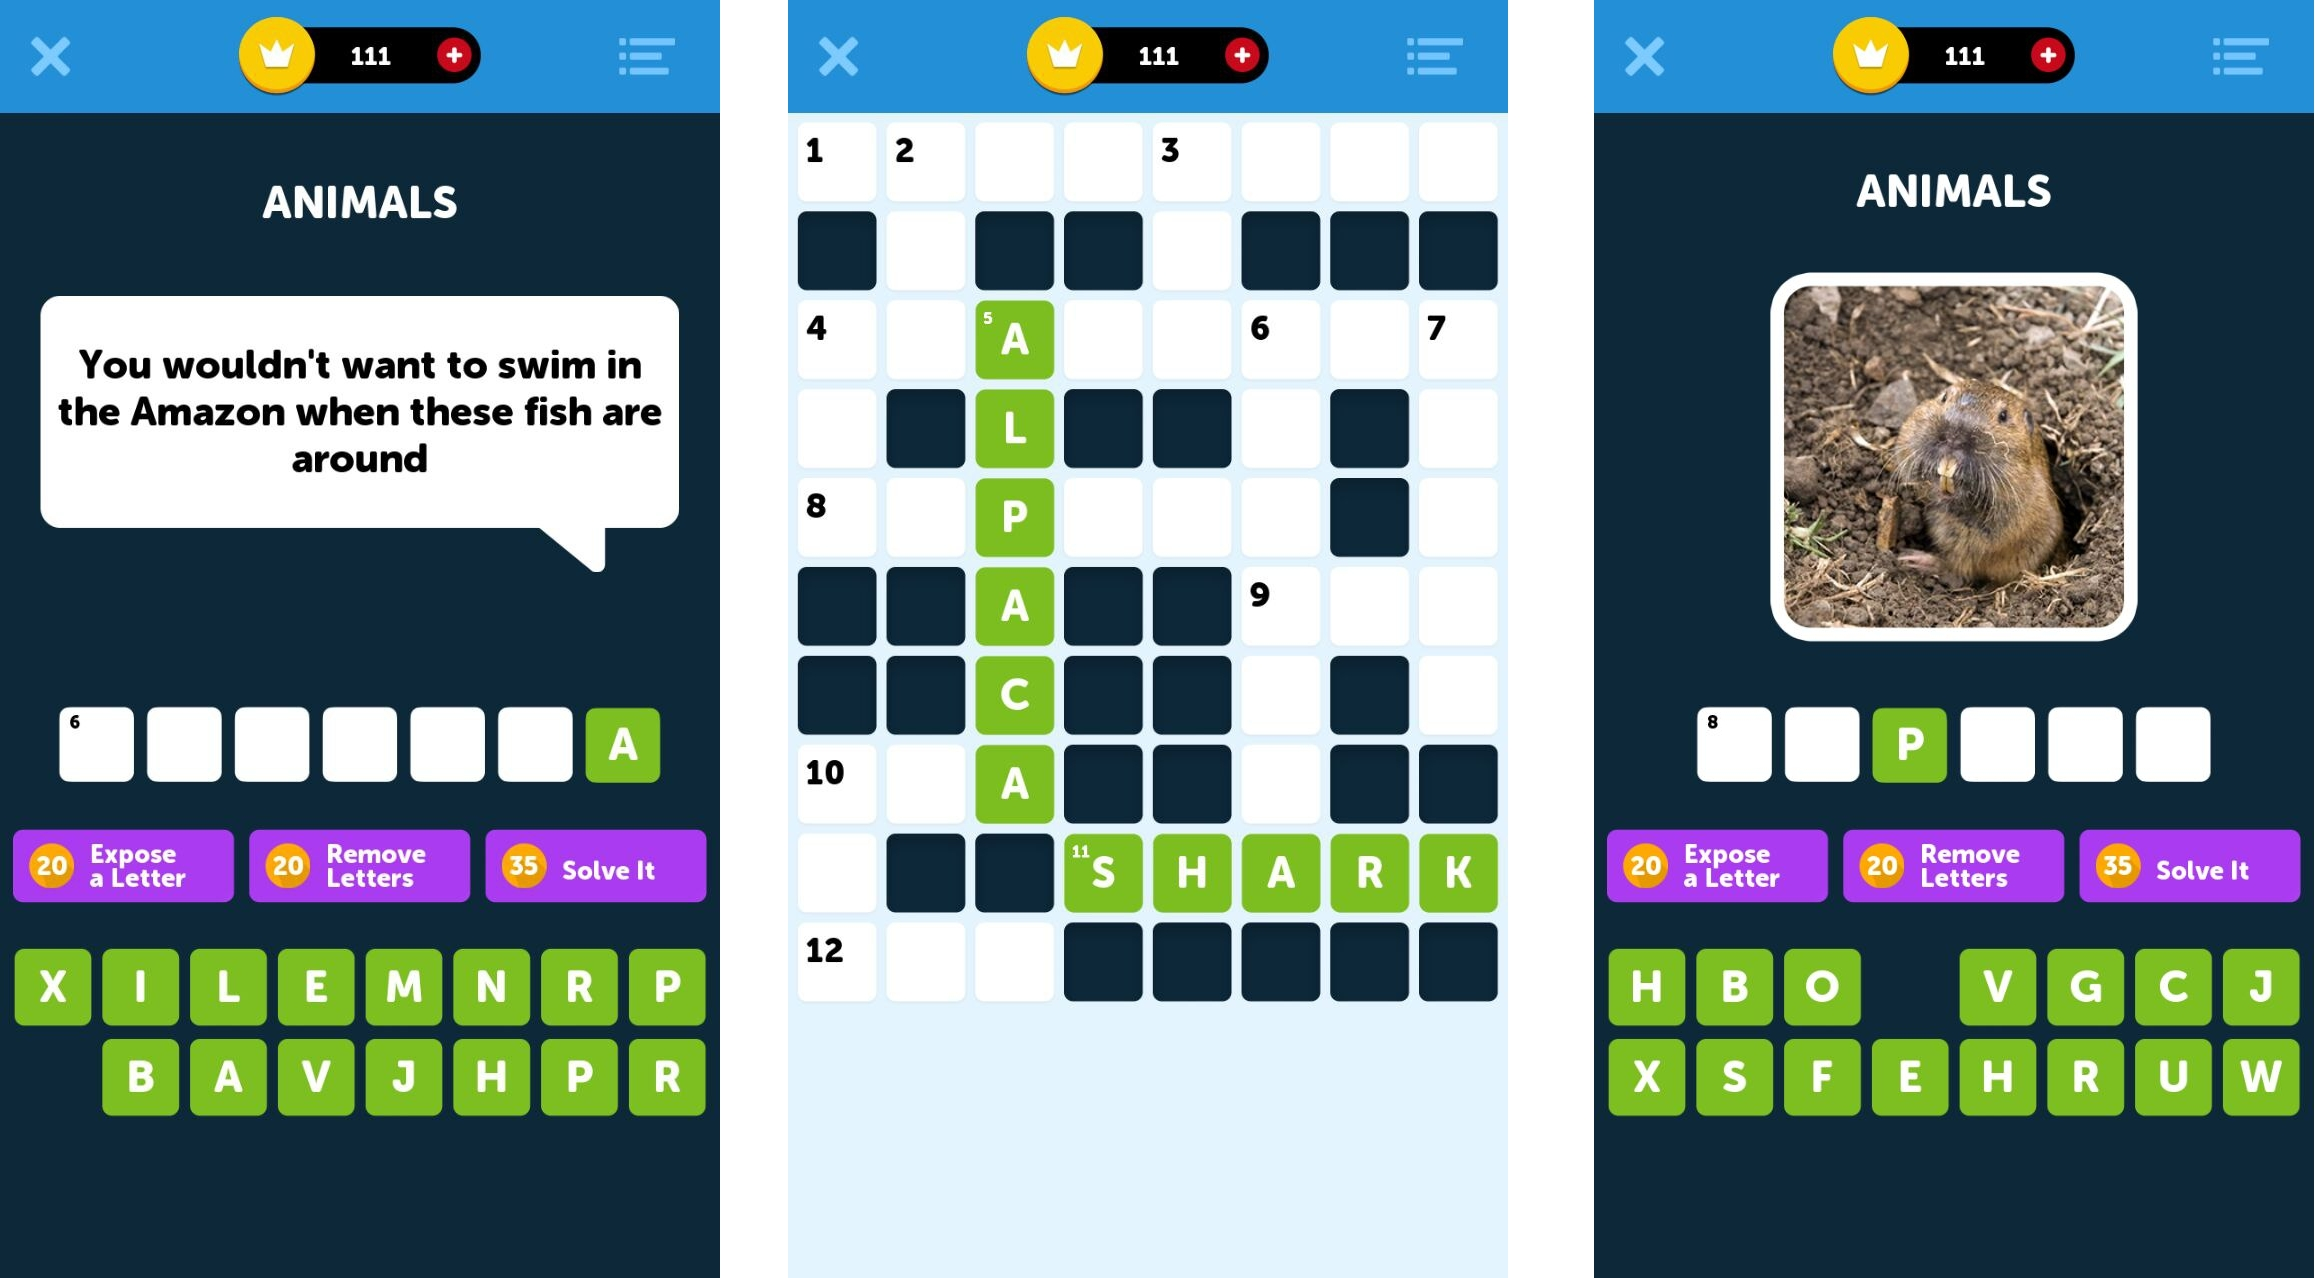
\includegraphics[width=0.9\textwidth]{Figuras/crosswordQuiz.jpg}
    
    Fonte: Elaborada pelo autor
\end{figure}

% inicio n deixe a vovó cair

\item[Não deixe a vovó cair]\footnote{\url{https://play.google.com/store/apps/details?id=com.GazGames.SalveVovo&hl=pt_BR}} \hfill \\
Não deixe a vovó cair (\autoref{fig:nDeixeVovoCair}) é um aplicativo que visa reduzir os riscos do ambiente domiciliar. Produzido pelo Centro de Telessaúde do Hospital das Clínicas – UFMG e pela Rede de Teleassistência de Minas Gerais, possui 4 níveis que representam áreas de uma casa: Banheiro, Quarto, Cozinha e Sala. Além disso, conta com a ajuda do cão Neca que representa o cachorro da dona e guia o usuário nos passos do jogo.
\begin{figure}[H]
\centering
    \caption{Telas do aplicativo \textit{Crossword Quiz}}
    \label{fig:nDeixeVovoCair}
    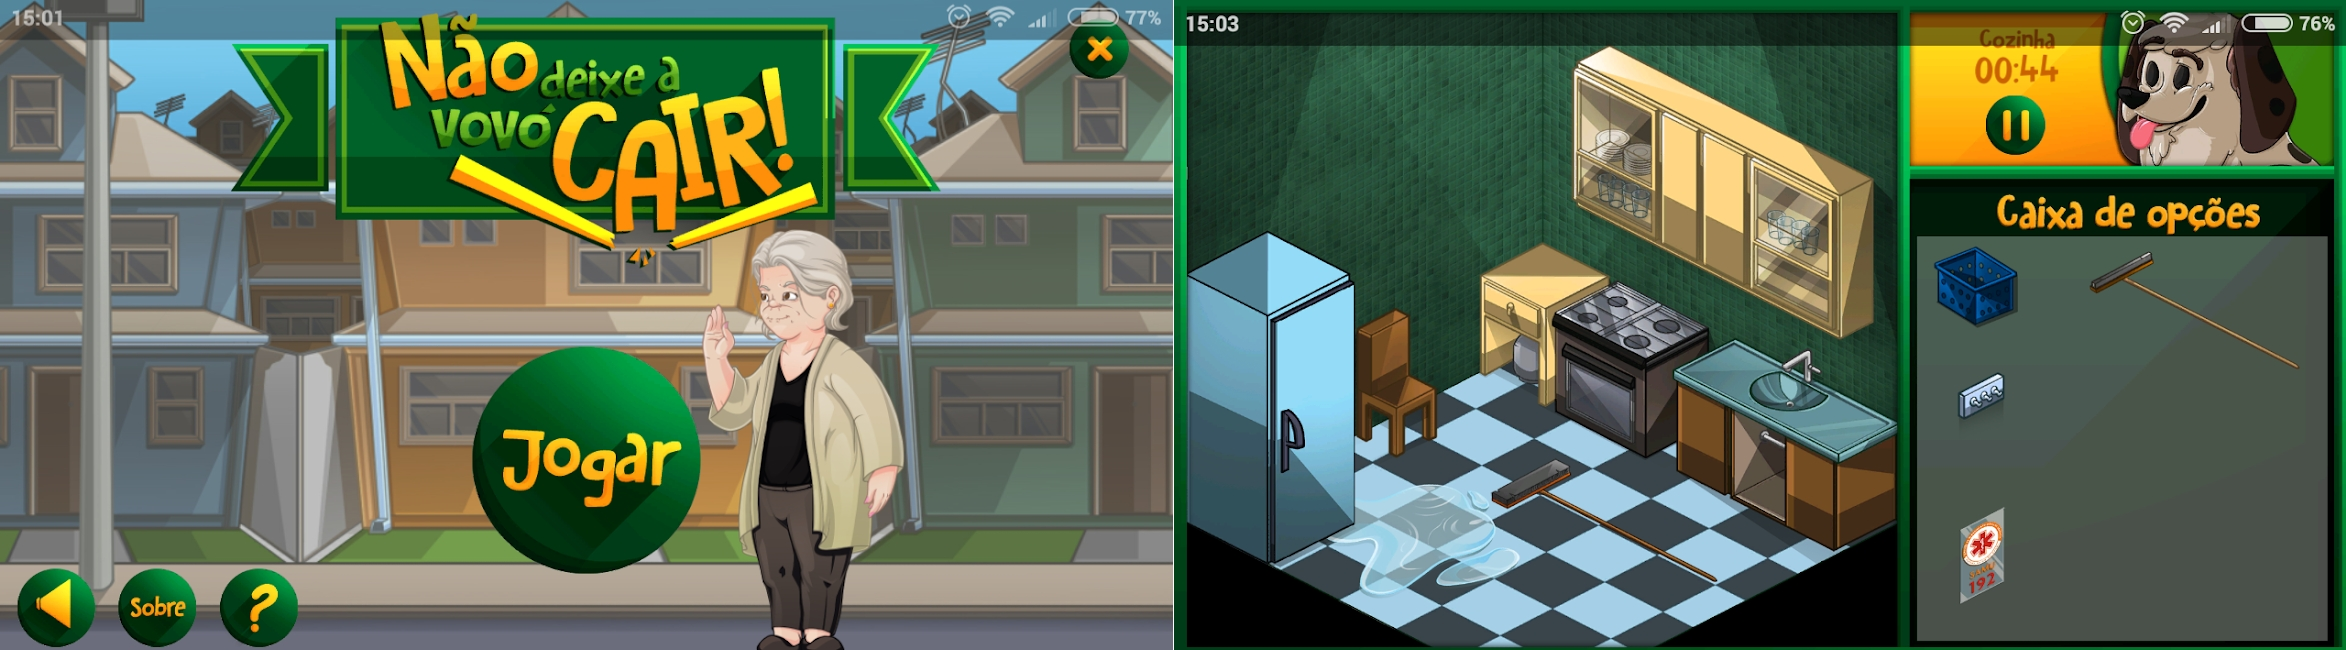
\includegraphics[width=0.9\textwidth]{Figuras/nDeixeVovoCair.jpg}
    
    Fonte: Elaborada pelo autor
\end{figure}

% fim

\end{description}


\begin{table}[!ht]
\caption{\textit{Funcionalidades das aplicações educacionais}}
\centering
\footnotesize
\begin{tabular}{p{6cm} p{12cm}}
\toprule
\textbf{Aplicativo} & \textbf{Funcionalidades}                                              \\ \midrule

Engaging congress   & \begin{tabular}[c]{@{}l@{}}Vídeos educativos\\ Perguntas relacionadas ao conteúdo\\ Nota após término dos exercícios\\ Botões de dúvida em todas as telas\end{tabular}                                                                 \\ \midrule
Play PBS KIDS Games & \begin{tabular}[c]{@{}l@{}}Funcionamento offline\\ Gerenciamento de consumo de memória\\ Obtenção de detalhes de desenhos passados na TV PBS Kids\end{tabular}      \\ \midrule
Human Anatomy Atlas & \begin{tabular}[c]{@{}l@{}}Interatividade com estruturas 3D\\ Mais de 1000 questões para testes\\ Realidade aumentada\\ Sete idiomas disponíveis\end{tabular}    \\ \midrule
Bini Super ABC & \begin{tabular}[c]{@{}l@{}}Aprendizado das letras por sons\\ Reforço do material aprendido\\ Controle de responsáveis para jogos\end{tabular}                \\ \midrule
Crossword Puzzle Free & \begin{tabular}[c]{@{}l@{}}Teclado não nativo, utiliza um personalizado\\ Dica acima do teclado\\ Botão de dica para a palavra\end{tabular}                \\ \midrule
Crossword Quiz & \begin{tabular}[c]{@{}l@{}}Não mostra o teclado todo, apenas algumas letras\\ Mostra imagens em vez de dicas em texto também\\ Tutorial inicial mostrando todos os passos antes da primeira partida\end{tabular}                \\ \midrule
Não deixe a vovó cair & \begin{tabular}[c]{@{}l@{}}Tutorial inicial ensinando o uso do aplicativo\\ Dicas em meio ao jogo para aplicações reais \\ Marcação do tempo para desafiar o usuário a melhorar cada vez mais \end{tabular}                \\ \midrule
\end{tabular}
\label{tab:sprint}
\end{table}


\section{Estudos sobre ensino para idosos}
blabla

\section{Estudo sobre os artefatos}
Nesta seção, será abordado o estudo feito de artefatos que auxiliam o desenvolvimento de aplicações educacionais móveis: as diretrizes de acessibilidade WCAG 2.1 e os padrões pedagógicos do ReqML-Catalog \citep{soad2017reqml}.

\subsection{Pesquisa sobre recomendações da WCAG 2.1}
A \textit{Web Content Accessibility Guidelines} \citep{wcag} é um conjunto de recomendações criadas pela \href{https://www.w3.org/}{W3C} com o objetivo de tornar o conteúdo da Web mais acessível para pessoas com deficiências tais como: cegueira ou baixa visão, surdez ou indivíduos com perda de audição, pessoas com limitações de movimentação, deficiências de fala, fotossensibilidade e limitações cognitivas. As recomendações abrangem \textit{desktops}, \textit{notebooks}, \textit{tablets} e dispositivos móveis, os quais são o foco desse projeto. É importante destacar que a versão 2.1 foi construída respeitando a versão 2.0, publicada em dezembro de 2008. O documento foi revisado pelos membros da W3C, desenvolvedores de software e por outros grupos interessados, os quais foram julgados capazes pela própria W3C. Os 4 princípios utilizados para a acessibilidade na Web são: perceptível, operável, compreensível e robusto.
\begin{itemize}
    \item Perceptível - Informações e componentes de interface do usuário precisam ser apresentadas de maneira que ele perceba
    \item Operável - Componentes da interface do usuário e navegação precisam ser operáveis
    \item Compreensível - Informações e as operações da interface do usuário devem ser compreensíveis
    \item Robusto - O conteúdo deverá ser robusto o suficiente para ser interpretado por uma variedade de agentes de uso, incluindo tecnologias de assistência
\end{itemize}

O WCAG possui três níveis de conformidade:
\begin{enumerate}
    \item Nível A: Pouco impacto no design
    \item Nível AA: Médio impacto no design
    \item Nível AAA: Muito impacto no design
\end{enumerate}

Embora a documentação oficial restrinja a aplicação dos níveis de conforidade a páginas web, ela ainda se mostrou importante para basear o impacto no design das telas do aplicativo. 
Serão destacados os critérios que mais influenciaram o desenvolvimento do aplicativo:

\begin{itemize}
    \item 1.2.2 Legendas (Nível A): Será disponibilizada a transcrição dos áudios e vídeos utilizados pelo aplicativo.
    \item 1.2.8 Mídias alternativas (Nível AAA): Além de ser disponibilizado o conteúdo em texto, também será oferecida a possibilidade de consumir o conteúdo em áudio ou vídeo.
    \item 1.4.3 Contraste mínimo (Nível AA): Serão respeitados os limites de contraste mínimo entre cores de 4.5:1.
\end{itemize}


\subsection{ReqML-Catalog}
O \textit{ReqML-Catalog} \citep{soad2017reqml} se trata de um catálogo de requisitos para Aplicações Educacionais Móveis. Ele foi proposto com o objetivo de propiciar um maior apoio na formulação de requisitos para aplicativos de educação, visto que muitos ainda possuem problemas e desafios a serem resolvidos. Além disso, de acordo com a pesquisa feita pelos autores, não havia um conjunto de requisitos completos e bem definidos para Aplicações Educacionais Móveis. É importante destacar que a última versão é uma evolução de outras anteriormente produzidas, as quais foram desenvolvidas a partir de literatura sistemática, revisões, e baseadas no conhecimento de especialistas do assunto. 
O \textit{ReqML-Catalog} possui uma estrutura hierárquica de três níveis: \textbf{Pedagógico}, \textbf{Social} e \textbf{Técnico}, como se pode ver na Figura \ref{fig:reqML}.

\begin{figure}[H]
\centering
    \caption{ReqML-Catalog}
    \label{fig:reqML}
    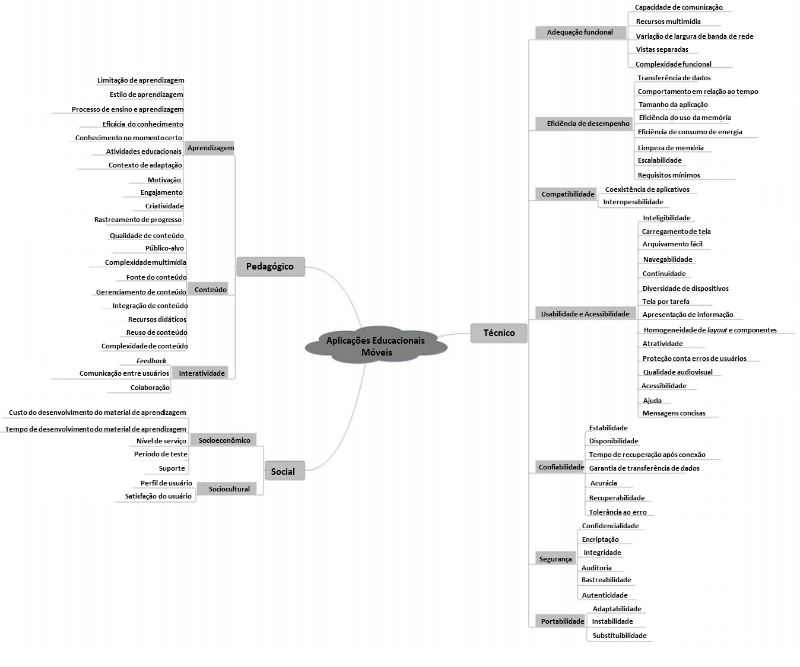
\includegraphics[width=0.9\textwidth]{Figuras/reqML-catalog.png}
    
    Fonte: \cite{soad2017reqml}
\end{figure}

As áreas que mais aproveitadas foram a Técnica e Social. Houve um maior destaque da área Pedagógica por dois motivos principais: forneceu um panorama mais aprofundado de elementos essenciais para a educação obtidos de especialistas e literaturas especializadas; uma vez que o foco do projeto é auxiliar a educação, mais atenção foi dada a esta área.

\section{Levantamento e estudo dos conceitos e tecnologias para desenvolvimento de aplicações móveis}

Nesta seção serão abordados os principais conceitos relacionados ao desenvolvimento de aplicações móveis. Desse modo, os principais temas foram: (i) estudo sobre Scrum e Requisitos que trata sobre a metodologia de desenvolvimento adotada neste projeto; (ii) estudos sobre React Native que contempla o levantamento e pesquisa da tecnologia adotada para concepção do sistema; (iii) por fim, estudos sobre UI/UX que discute o conhecimento relacionado a interface e experiência do usuário.

\subsubsection{Estudos sobre Scrum e Requisitos} 
Em 2001, um grupo de 17 pessoas se reuniu para discutir a respeito de desenvolvimentos mais leves de software, pois acreditavam que os modelos em voga eram lentos e burocráticos. O resultado foi o Manifesto Ágil \citep{agileManifesto}, em que os participantes propuseram princípios a serem seguidos. Segundo os criadores, deveria haver a valorização de: (i) Indivíduos e interações mais que processos e ferramentas; (ii) Software em funcionamento mais que documentação abrangente; (iii) Colaboração com o cliente mais que negociação de contratos; (iv) Responder a mudanças mais que seguir um plano.

Dentre os artefatos do \textit{Scrum}, devem ser citados o \textit{Product Backlog} e o \textit{Sprint Backlog}. O \textit{Product Backlog} possui todas as funcionalidades necessárias para o funcionamento do produto, as quais são ordenadas por prioridade. Já o \textit{Sprint Backlog} reúne as funcionalidades que serão desenvolvidas na atual \textit{Sprint} em execução.

Os eventos do Scrum são: (i) Sprint; (ii) Reunião de Planejamento da Sprint; (iii) Reunião Diária; (iv) Revisão da Sprint; (v) Retrospectiva da Sprint.

A \textbf{\textit{Sprint}} é essencial para o Scrum, durante um período de 2 a 4 semanas são desenvolvidas as atividades do \textit{Sprint Backlog}, as quais foram previamente selecionadas do \textit{Product Backlog}. Estas atividades são escolhidas na \textbf{Reunião de planejamento da \textit{Sprint}}. É importante destacar que concomitantemente à Sprint são realizadas \textbf{Reuniões diárias}, que possuem o objetivo de reunir o time de desenvolvimento a fim de sincronizar as atividades e criar um plano para as próximas 24 horas. Ao final do período separado para o incremento do produto, ocorre a \textbf{Revisão da Sprint}, com o objetivo de discutir o que foi feito, inspecionar o incremento e adaptar o \textit{Product Backlog}. A \textbf{Retrospectiva da Sprint} ocorre depois da Revisão da Sprint e antes da Reunião de planejamento da próxima Sprint, e é a oportunidade para o Time Scrum inspecionar a si próprio criar um plano para melhorias a serem aplicadas na próxima Sprint.

Ademais, existem funções diferentes para os membros chamadas de papéis. São eles: \textit{Product Owner}; Time de Desenvolvimento e \textit{Scrum Master}. 
O \textit{Product Owner}, ou dono do produto, se encarrega de maximizar o valor do produto e gerenciar os \textit{Backlogs}. O Time de Desenvolvimento concentra os profissionais responsáveis pelos incrementos do produto. Por fim, o \textit{Scrum Master} orquestra toda a equipe e deve garantir que o Scrum seja entendido e aplicado.

Outro fator importante para o desenvolvimento de um software são os requisitos. De acordo com \cite{Sommervile2010}, eles podem ser definidos como os serviços que o sistema promove, as restrições de operação e as descrições do que o sistema deveria realizar. É importante destacar a Engenharia de Requisitos, a qual fornece mecanismos apropriados para o entendimento da demanda do consumidor, análise de suas necessidades, avaliação da viabilidade, negociação de uma solução, especificação de uma solução não ambígua, validação da especificação e gerenciamento de requisitos enquanto são transformados em um sistema operacional \citep{Pressman2014}. 

Três são os principais tipos de requisitos \citep{Sommervile2010}:
\begin{itemize}
    \item \textbf{Requisitos funcionais}: são declarações de serviços que o sistema deve prover, como o sistema deve reagir a determinados tipos de entrada, e como deveria funcionar em situações particulares. Em alguns casos, os requisitos funcionais podem também explicitar o que o sistema não deveria fazer.
    
    \item \textbf{Requisitos não funcionais}: são restrições dos serviços ou funções oferecidos pelo produto. Incluem restrições de tempo, de processos de desenvolvimento, e restrições impostas por padrões. Requisitos não funcionais frequentemente se aplicam ao sistema como um todo, em vez de se aplicar a serviços ou \textit{features} individuais.
    
    \item \textbf{Requisitos de domínio}: são derivados do domínio de aplicação do sistema, e não de necessidades específicas de usuários do sistema. Podem ser novos requisitos funcionais, restringindo os já existentes. 
\end{itemize}


\subsection{Estudos sobre React Native} 
São diversas as maneiras de desenvolver um aplicativo móvel. A maneira convencional é utilizar a linguagem nativa: Java (Android) e Swift/Object-C (iOS), todavia isso causa o empecilho de se disponibilizar o aplicativo apenas para uma plataforma. Ainda, é possível usar \textit{frameworks} híbridos que recorrem ao uso de \textit{web-views} para renderizar a aplicação e disponibilizar para os dois sistemas operacionais, pode-se citar Ionic, Titanium, e PhoneGap. Entretanto, o desempenho de aplicativos construídos com tais tecnologias é precário. Pensando no problema, durante a conferência do React.js em 2015, o Facebook introduziu seu novo \textit{framework} React Native, o qual prometia revolucionar a maneira de desenvolver aplicativos móveis. A premissa era simples, possibilitar o desenvolvimento \textit{mobile} sem a necessidade de programação diferente para os dois sistemas operacionais líderes.

% Vantagens e desvantagens
As principais vantagens do uso do React Native, de acordo com \cite{danielsson2016}, são: (i) O desenvolvimento ocorre em uma única linguagem, sendo possível utilizar o aplicativo em iOS ou Android; (ii) A documentação oficial dá grande suporte de ajuda; (iii) O React Native não possui nenhum efeito negativo na experiência do usuário, pois a diferença de desempenho é imperceptível para a grande maioria dos usuários.

Dentre as desvantagens, é importante destacar: (i) Incerteza da possibilidade de executar frequentes tarefas em segundo plano quando o aplicativo já está sendo executado em segundo plano \citep{sodebergJohansson}; (ii) Testes concluem que a frequência GPU, carregamento de CPU, uso de memória e consumo de energia são levemente inferiores ao desenvolvimento nativo \citep{danielsson2016}.

Entretanto, embora existam algumas desvantagens do uso do React Native, em termos gerais é uma excelente alternativa para o projeto, pois não compromete de maneira significante a performance do aplicativo e possibilita o uso nas plataformas iOS e Android, alcançando assim, um número maior de usuários.

\subsection{Estudos sobre UI/UX}
A Interface de Usuário (UI) se refere a um sistema e um usuário interagindo um com outro por meio de comandos para operar o sistema, inserir dados, e usar o conteúdo \citep{joo2015}. Já a Experiência de Usuário (UX), segundo \cite{marc2008}, é uma perspectiva distinta da qualidade de tecnologia interativa. O autor ainda define UX como uma avaliação momentânea e primária da sensação (bom-ruim) enquanto interage com o produto ou serviço. Dessa forma, UX troca a atenção dos produtos e materiais para as sensações humanas - o lado subjetivo do uso do produto. Ainda, de acordo com \cite{castilla2017}, a UX representa uma mudança do próprio conceito de usabilidade, pois o objetivo não se reduz a melhorar a sensação do usuário na eficácia, eficiência e facilidade de aprendizagem, mas sim tentar resolver o problema estratégico da utilidade do produto para o usuário. 

Dessa maneira, pode-se concluir que a interface e experiência do usuário cumprem papéis essenciais no desenvolvimento de um produto, sendo indispensável seu planejamento. Ainda, tendo em vista o público alvo do atual projeto, usuários idosos, torna-se necessária a atenção e cuidado no assunto a fim de alcançar os objetivos finais.

Portanto, tendo em mente os motivos acima citados, foi realizado um minicurso sobre a Experiência de usuário e Interface de usuário com uma especialista da área UI/UX cujo título era ``Como incluir UX e UI Design nos seus projetos''. A realização se deu na 22ª Semana da Computação da Universidade de São Paulo, campus de São Carlos, no dia 03/10. O minicurso se mostrou de grande importância, uma vez que possibilitou a expansão do conhecimento do assunto em termos práticos, sendo possível sua aplicação no projeto.

\section{Desenvolvimento}
blabla

\subsection{Estudo do primeiro algoritmo de geração das palavras cruzadas} 
Nesta subseção será abordado o primeiro algoritmo de geração das palavras cruzadas estudado, o qual necessita de um grande banco de palavras para ser executado corretamente. Para melhor compreensão deste, é essencial a noção dos paradigmas clássicos da Ciência da Computação: Força Bruta e \textit{Backtracking}. Além disso, é interessante uma pequena noção das Cadeias de Markov Absorventes.

A Força Bruta é um paradigma de programação em que o espaço de busca é vasculhado sistematicamente até que se encontre a solução desejada.

Já o \textit{Backtracking} é também um paradigma de programação largamente estudado nos cursos de Ciência da Computação. Segundo \cite{nilsson1980principles}, o \textit{Backtracking} é um método de resolução de problemas de Ciência da Computação em que se estende incrementalmente uma solução parcial que especifica valores consistentes para uma das variáveis, em direção a uma solução completa, ao repetidamente escolher um valor para outra variável consistente com os valores da atual solução parcial.

Define-se Cadeias de Markov como um Processo de Markov com a seguinte propriedade: qualquer comportamento futuro do processo, quando seu estado atual é conhecido com exatidão, não é alterado por nenhum conhecimento adicional em relação aos comportamentos passados \citep{howard1998introduction}. Caso a cadeia possua no mínimo um estado final de absorção em que seja possível chegar, é chamada Cadeia de Markov Absorvente.

O algoritmo utilizado é intitulado \textit{Wizium} \citep{wizium}.

A primeira abordagem para a solução do problema seria simplesmente utilizar o paradigma da Força Bruta.

\begin{figure}[H]
\centering
    \caption{Árvore de tentativas utilizando Força Bruta}
    \label{fig:crossTree}
    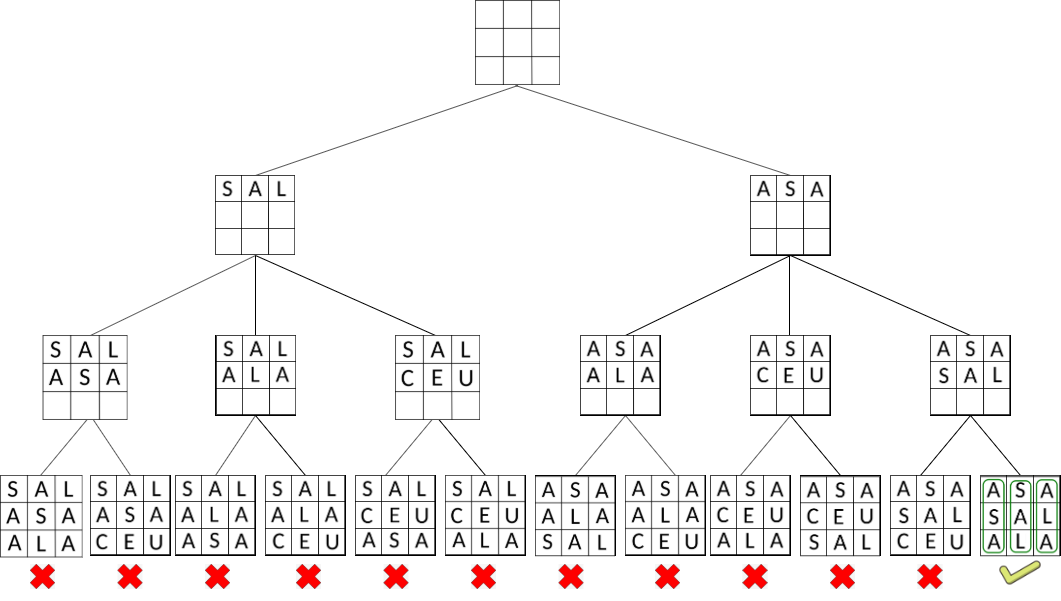
\includegraphics[width=0.9\textwidth]{Figuras/crosswordsTree.png}
    
    Fonte: Elaborada pelo autor
\end{figure}

Como pode-se perceber, a análise só é feita após o último passo. Algumas ramificações da árvore de tentativas poderiam ter sido ``podadas'' com uma análise prévia do tabuleiro antes que chegasse em seu estado completo.   

Portanto, faz-se necessária uma abordagem mais elaborada utilizando-se o \textbf{entrelaçamento}, como se pode observar na Figura \ref{fig:entrelacamento}. 

\begin{figure}[H] 
\centering
    \caption{Inserção de palavras por entrelaçamento}
    \label{fig:entrelacamento}
    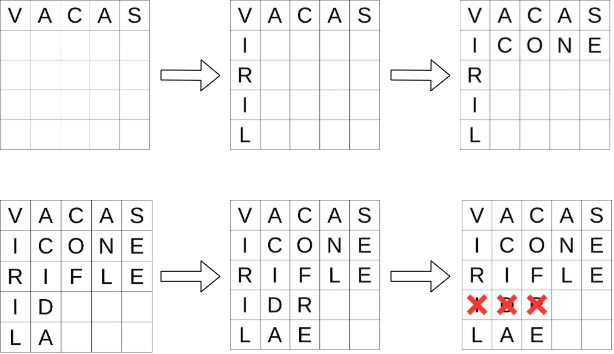
\includegraphics[width=0.9\textwidth]{Figuras/entrelacamento.jpg}
    
    Fonte: Elaborada pelo autor
\end{figure}

Dessa maneira, será possível eliminar o quanto antes ramificações que não poderão gerar uma solução para o problema.

Será a feita a modelagem do problema como um Processo Estocástico. Como está sendo utilizada a aproximação da probabilidade de coincidência de letras para palavras quaisquer,
% ($p_{co}$ \ref{pco})
é conveniente aproximar cada estado do Processo como a tentativa de inserção de uma palavra na horizontal ou vertical. Haverão as possibilidades de sucesso ou falha do processo; caso seja possível inserir uma palavra ocorrerá o avanço, caso contrário, o retrocesso ao estado anterior utilizando-se o \textit{Bactracking}. 

Sem perdas de generalidade, seja N a quantidade de palavras de tamanho S no banco de palavras, $wh_{i}$ e $wv_{i}$ as S células horizontais e verticais, respectivamente. A probabilidade de que seja possível a inserção em uma palavra na posição $i$ é dada por:

\begin{center}
    \Large{$p_{hi} = 1 - (1 - p_{co}^{i})^{N}$}
    
    \Large{$p_{vi} = 1 - (1 - p_{co}^{i+1})^{N}$}
\end{center}

Onde $i = 0...S-1$. De maneira mais clara, são as probabilidades de uma palavra inserida na vertical ou horizontal tenha a coincidência de letras até a posição $i$. Portanto, a modelagem do problema se reflete na seguinte Cadeia de Markov:

\begin{figure}[H]
\centering
    \caption{Cadeia de Markov para entrelaçamento}
    \label{fig:markov1}
    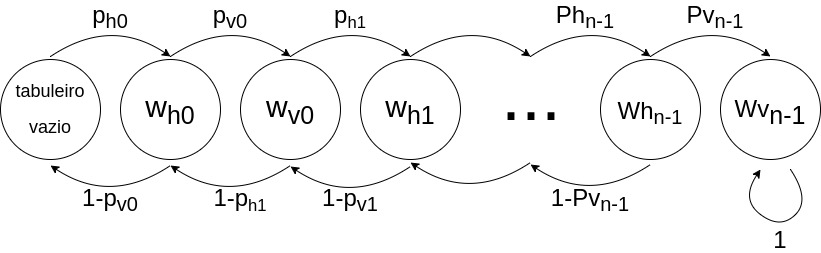
\includegraphics[width=0.9\textwidth]{Figuras/markovChain1.jpg}
    
    Fonte: Elaborada pelo autor
\end{figure}

% Decidir se vai colocar o passo a passo ou mesmo a tabela (isso abaixo) no relatorio
% Utilizando-se os conceitos de tempo médio para o estado de absorção expostos anteriormente, é possível calcular a quantidade de passos média do algoritmo de \textit{Bactracking} até que se chegue em uma solução.

% Colocar tabela de passos (e talvez) com o tempo de execução em segundos, minutos, etc

Todavia, ainda é possível aumentar a eficiência do algoritmo antecipando ainda mais os ramos da árvore de tentativas que não poderão gerar uma solução. O algoritmo anterior verifica a possibilidade de inserção de uma palavra examinando até a posição $i$, não considerando com antecedência impossibilidades das linhas ou colunas , como na Figura \ref{fig:scaffolding}, que tem a última coluna sendo iniciada com \textbf{SR} (palavras de 5 letras iniciadas com \textbf{SR} são inexistentes no banco de palavras usado). Dessa maneira, diversos passos ainda são executados mesmo com uma formação impossível de tabuleiro, desperdiçando tentativas e tempo de computação.


% Colocar aqui aquele que só da PS na ultima vertical
\begin{figure}[H]
\centering
    \caption{O algoritmo só detectaria a impossibilidade da última coluna no último passo}
    \label{fig:scaffolding}
    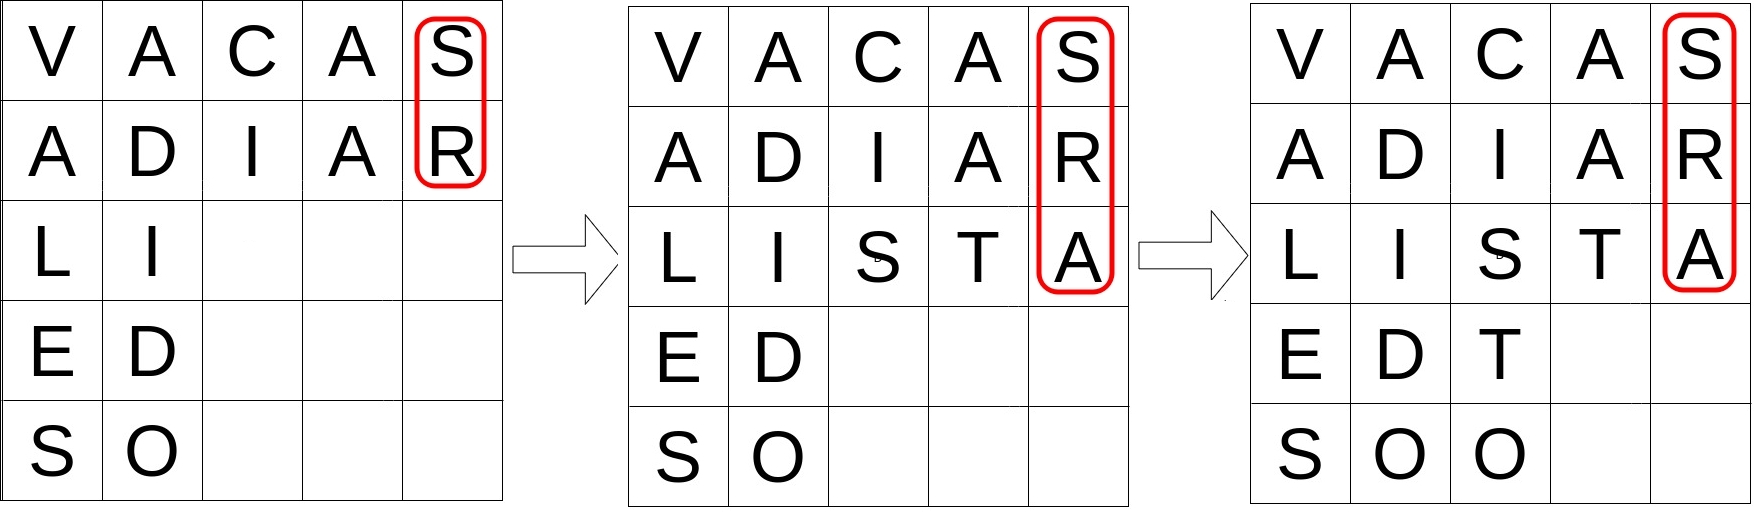
\includegraphics[width=0.9\textwidth]{Figuras/bradingerror.jpg}
    
    Fonte: Elaborada pelo autor
\end{figure}

Logo, verificar a possibilidade de inserir palavras na vertical nas S posições solucionaria o problema acima descrito, pois anteciparia ainda mais os ramos da árvore sem solução. A nova abordagem consiste em inserir uma palavra na horizontal, se e somente se, houverem prefixos compatíveis cujas palavras possam ser inseridas em cada uma das posições verticais.

\begin{figure}[H]
\centering
    \caption{Verificando cada posição vertical}
    \label{fig:scaffoldingcool}
    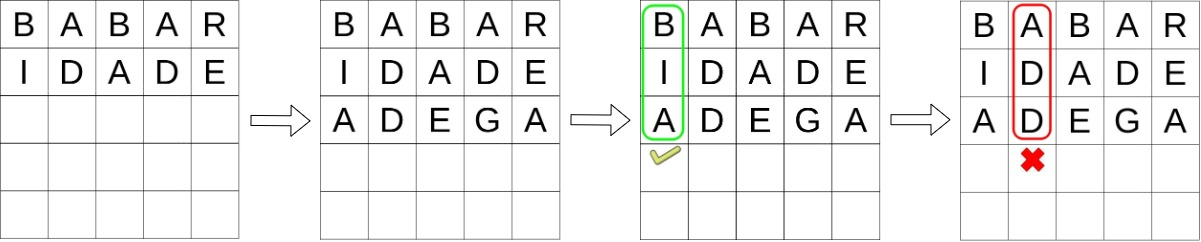
\includegraphics[width=0.9\textwidth]{Figuras/scaffoldingcool.jpg}
    
    Fonte: Elaborada pelo autor
\end{figure}

% Obs.: Em vez de retornar o número médio de palavras de tam S com prefixo i; eu nao deveria retornar o quantidade total de palavras com tamanho maior ou igual a i?
Seja $M(S,i)$ a função que retorna o número médio de palavras de tamanho $S$ que possuem prefixo de tamanho $i$. Portanto, é possível definir a probabilidade de existir uma palavra que possa ser inserida na vertical ao se colocar uma letra na posição $i$; só é necessário verificar a última letra pois as $i-1$ letras anteriores já foram testadas previamente.

\begin{center}
    \Large{$p_{co_{i}} = M(S,i)*p_{co}$}
\end{center}

Logo, a probabilidade de uma palavra poder ser inserida na horizontal na linha $i$ é dada por:

\begin{center}
    \Large{$p_{h_{i}} = N*(p_{co_{i}})^{S}$}
\end{center}

Como comentado anteriormente, o algoritmo necessita de um grande banco de palavras para ser executado da maneira esperada. Dessa maneira, possíveis aplicações futuras poderão surgir; todavia, para o período coberto por este relatório o foco de desenvolvimento foi dado ao segundo algoritmo, que será elucidado na subseção seguinte.

\subsection{Estudo do segundo algoritmo de geração de palavras cruzadas}
Nesta seção será abordado o segundo algoritmo de geração de palavras cruzadas, o qual será utilizado no projeto do aplicativo. Uma lista de palavras é dada para que se gere uma palavra cruzada formada somente por estas. Portanto, a abordagem se torna diferente do primeiro algoritmo analisado, o qual utiliza um grande banco de palavras para gerar o tabuleiro.

O usuário pode escolher o tamanho do tabuleiro, caso uma palavra seja grande demais e não consiga ser inserida, ela é eliminada da lista e não segue para os próximoas passos.

O algoritmo inicia gerando uma tabela com o mesmo número de colunas e linhas. Essa quantidade é definida multiplicando-se o tamanho da maior palavra por um fator definido como 3. Por exemplo, caso a maior palavra tenha 7 letras e o fator seja 3, será gerada uma tabela 14x14. Isso ocorre para aumentar a probabilidade de interseção entre palavras. 

Após estas etapas, é iniciado o procedimento de inserção. É feita a tentativa de inserção para cada uma das palavras fornecidas em todas as posições possíveis do tabuleiro iniciando-se com a disposição horizontal e após a vertical. Caso ocorra algum conflito da palavra inserida com outra que já esteja no tabuleiro, a posição será ignorada. Uma terminada a tentativa de inserção de uma palavra em todas as posições, é feita a análise de pontuação entre elas. Apenas a posição que possuir a maior pontuação permanecerá. Para isso, são computados quatro tipos de pontuações, como mostrado na (\autoref{fig:codeScores}). As avaliações possuem os seguintes pesos percentuais:

\begin{itemize}
    \item Número de conexões - 70\%
    \item Distância do centro do tabuleiro - 15\%
    \item Tamanho da palavra - 5\%
    \item Vertical vs Horizontal - 10\%
\end{itemize}

\begin{figure}[H]
\centering
    \caption{Funções de avaliação de pontuações do tabuleiro}
    \label{fig:codeScores}
    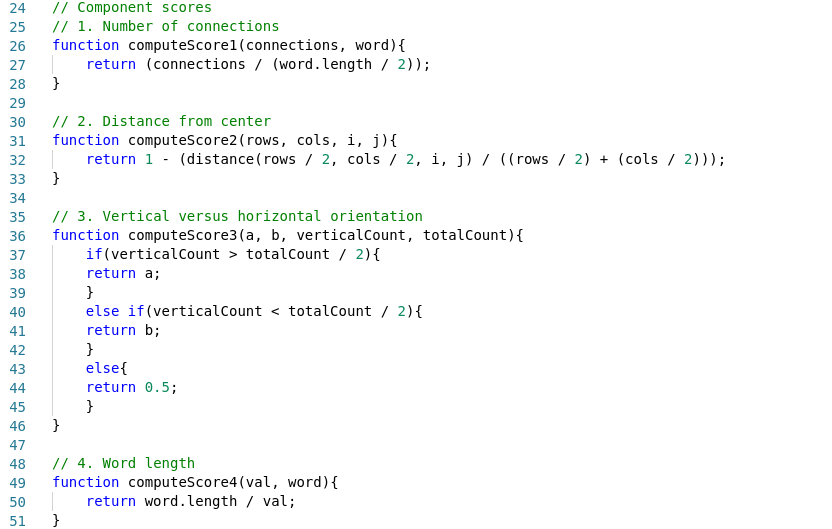
\includegraphics[width=0.9\textwidth]{Figuras/codeComponentScores.png}
    
    Fonte: \cite{layoutGenerator}
\end{figure}

O último fator tenta equilibrar a quantidade de palavras na horizontal e na vertical. Caso mais da metade das palavras já inseridas estiver na horizontal e a palavra que está sendo analisada no momento estiver na vertical, ela é melhor avaliada.

Uma vez que a palavra é inserida armazena-se sua posição no tabuleiro, bem como sua orientação vertical ou horizontal e seu tamanho.

Esse processo é feito com todas as palavras da lista. Todavia, pode ocorrer o caso de uma palavra fica isolada sem interseções. Assim, todas essas são eliminadas. É importante lembrar que o tabuleiro está em um tamanho maior do que o desejado pelo usuário, pois no início ocorreu uma expansão das linhas e colunas ao multiplicá-las por um fator que havia sido definido como 3. Dessa maneira, restam colunas e linhas que estão vazias e podem ser eliminadas. Logo, o último passo é reduzir o tabuleiro para seu tamanho ideal respeitando o desejado pelo usuário. O algoritmo exporta um arquivo JSON contendo as palavras, suas orientações, posições e tamanho.

\subsection{Desenvolvimento do MVP}
% Escrever o que foi feito em termos de desenvolvimento técnico {
%     - Colocar algumas linhas de código
%     - Falar de alguns desafios do React Native
%     - Explicar a arquitetura do React Native do app
% }
Nesta subseção será abordado o processo de elaboração do MVP em termos técnicos bem como a arquitetura básica dos softwares utilizados.
O desenvolvimento se deu utilizando o   \textit{\href{https://reactnative.dev/}{React Native}}, que permite a construção de aplicativos para Android e iOS.

Duas telas foram utilizadas para o teste interligadas por uma navegação em \textit{Stack}. A primeira possibilita a escolha do tamanho do tabuleiro bem como o tema de cores. Já a segunda é a própria tela do jogo de palavras cruzadas, em que se encontra o tabuleiro, o teclado personalizado e a dica das palavras.

Decidiu-se para a construção do MVP de teste utilizar apenas um conjunto de palavras para construção das palavras cruzadas, a fim de focar nas questões de usabilidade e acessibilidade.

A tela de jogo foi desenvolvida da seguinte maneira: uma \textit{tag} \textit{<View>} comporta quatro \textit{tags} principais nativas do \textit{React Native}:

\begin{itemize}
    \item \textit{<FlatList>}, responsável por renderizar as células do tabuleiro
    \item \textit{<View>}, responsável por encapsular as também nativas \textit{tags} \textit{TouchableOpacity}. Em conjunto se tornam a seção que mostra a dica da resposta para a palavra selecionada 
    \item \textit{<View>}, que encapsula o componente customizado \textit{<Keyboard>}, o qual renderiza o teclado personalizado
    \item \textit{<Modal>}, que fica invisível até que o usuário decida expandir o texto da dica
\end{itemize}

O teclado personalizado foi introduzido por termos de acessibilidade, botões maiores permitem uma melhor experiência para o usuário idoso. É importante destacar que ele é formado pelas letras que compõem a palavra a ser preenchida acrescida de letras aleatórias.

Para algumas mudanças de informação na tela de jogo, decidiu-se utilizar a \textbf{Manipulação Direta} (\href{https://reactnative.dev/docs/direct-manipulation}{\textit{Direct Manipulation}} de acordo com a documentação oficial) pois evita-se a renderização de toda a tela para pequenas mudanças, o que poderia acarretar problemas de desempenho. Dessa maneira, o estado dos componentes é modificado por meio de referência, acarretando em um melhor desempenho. Os componentes que recebem a Manipulação Direta são \textit{<Tiles>}, que são os componentes customizados os quais renderizam as células do tabuleiro. Ocorrem duas Manipulaçoes Diretas com esses componentes: alteração do foco e substituição da letra exibida.

Na Figura \ref{fig:codeDirectManipulation} podemos ver a função \textit{inputLetter}, que recebe como argumento uma letra. O trecho do código promove uma mudança do valor de uma propriedade no componente em que se faz a referência. Cada célula do tabuleiro está armazenada em uma matriz, para acessá-la utiliza-se \textit{this.ref[posicaoI][posicaoJ]}. Nas linhas 208, 209 e 210 ocorre a mudança da propriedade \textit{text}, seu novo valor passará a ser o armazenado na variável \textit{letter}, a qual é recebida diretamente do teclado personalizado.

\begin{figure}[H]
\centering
    \caption{Método que utiliza manipulação direta}
    \label{fig:codeDirectManipulation}
    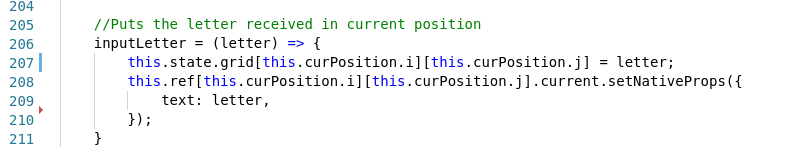
\includegraphics[width=0.9\textwidth]{Figuras/codeDirectManipulation.png}
    
    Fonte: Elaborada pelo autor
\end{figure}

As mudanças de estado que que ocorrem na tela de jogo são:

\begin{itemize}
    % informal por enquanto
    \item substituição de letra no tabuleiro
    \item mudança de cor para a célula que possui o foco
\end{itemize}